\documentclass[]{article}
\usepackage[a4paper, total={6in, 8in}]{geometry}
\usepackage{booktabs}
\usepackage{multicol}
\usepackage[sorting=none,sortcites=true,backend=bibtex]{biblatex}
\bibstyle{numeric-comp}
\bibliography{bibliography}

\newcommand{\todo}[1]{{\color{red}[\textit{TODO: #1}]}}

\usepackage{tikz}
\usetikzlibrary{shapes.geometric, arrows}

\tikzstyle{process} = [rectangle, 
minimum width=12cm, 
minimum height=1cm, 
text width=11cm, 
draw=black, 
fill=white,
rounded corners]

\tikzstyle{subprocess} = [rectangle, 
minimum width=5cm, 
minimum height=0.6cm, 
text centered, 
text width=5cm, 
draw=black, 
fill=white]

\tikzstyle{arrow} = [thick,->,>=stealth]

\begin{document}
\section{Introduction}
Electrification  of public transport has become the norm over recent years. Many public transport poviders, such as the Dutch bus provider Qbuzz \cite{qbuzzQbuzz}, have been replacing traditional vehicles with electric vehicles (EVs) in their fleet with the aim of reducing their carbon footprint in order to match the stricter regulations set out by organizations such as the European Union \cite{europaRegulation20181999}. This electrification introduces new challenges in every step of the planning process, as can be seen in Figure \ref{fig:planning-overview}. The limits of both electric infrastructure and electric vehicles add new constraints to an already complex operation. Existing techniques that minimize operational costs therefore need to be revised in order to add consideration for these new constraints. \\\\
In this work, we focus on two of the most costly steps of the planning process for busses: vehicle scheduling and crew scheduling. Crew scheduling in particular is of great importance, as this makes up a majority of the overall operational costs \cite{BODIN198363}. A recent estimate puts crew costs at circa $60\%$ of the total operational costs for bus companies in Northern Europe \cite{PERUMAL2019280}. \todo{uitbreiden} \\\\
The Vehicle Scheduling Problem (VSP) aims to find a set of minimum cost vehicle tasks such that all trips that need to be driven throughout a timeperiod are covered. In this, a trip is defined as full or partial travel of a vehicle along a predetermined route, and a vehicle task is defined as a set of sequential operations that a vehicle will perform. Note that for the same route, multiple trips might be present on a single day if that route is scheduled multiple times. \\
Given a set of these trips, a set of depots used to store vehicles that are not in use, and a set of vehicles, the goal is to find a vehicle task (or schedule) for each of the vehicles throughout the day. In this, a task for an individual vehicle must start at a depot, perform a number of compatible trips (that is, trips which can be performed sequentially while respecting driving times between trips), before finally returning to its original depot. In order to minimize operational costs, both the number of vehicles and the overall driven distance between trips (also called deadheads) need to be minimized. \\
The VSP with a single depot and unconstrained vehicle ranges can be solved in polynomial time \cite{Freling2003SDVSP}. The multi-depot variant of the problem on the other hand is known to be NP-hard \cite{BODIN198363, Bertossi1987, Even1975}, and the addition of constrained vehicle ranges such as those found in EVs also make the problem NP-hard \cite{BODIN198363, Sassi2014}. As we consider a general depot case with constrained vehicle ranges due to the inclusion of EVs we will refer to the VSP as being NP-Hard. \\\\ 
The Crew Scheduling Problem (CSP) aims to find a minimum cost assignment of crew members to vehicle tasks. Given a set of vehicle tasks and crew members, the goal is to find an assignment of crew members such that each vehicle is always driven by exactly one driver. In this, constraints such as maximum working time on a day, driver breaks and handovers between different drivers on the same vehicle need to be considered. The primary goal for minimization here is the total amount of workers needed and hours worked. The CSP is also known to be an NP-hard problem \cite{Fischetti1989}.\\\\
As can be seen, the VSP and CSP are closely related. The vehicle schedules that are selected in the VSP directly determine the crew assignments which are possible within the CSP. It is therefore not always optimal to fully minimize costs in the vehicle scheduling process, as this might incur higher costs during crew scheduling. The need for an approach which combines the two problems was already recognized in ... by .... \todo{cite needed}, with the aim of further reducing operational costs. This integrated approach is often refered to as the vehicle and crew scheduling problem, or VSCP. \\\\
A lot of work has already been for these three problems. Both the sequential and integrated approach have been extensively studied since the \todo{1980s?}, and we refer the reader to a recent survey in order to get a sense of the current state of the art \todo{citiation met survey}. The introduction of electric vehicles has however introduced new constraints. The most important constraint is the limited range of these vehicles, combined with charging times which are much greater than refeuling times found on traditional busses. This most directly effects the VSP, as charging periods now need to be added throughout the day in order to effectively use busses. This new version of the problem, refered to as the E-VSP (as well as E-CSP and E-VCSP for the other problems respectively) has also been studied in the past. We once again refer the reader to a survey by Perumal et al. a more cohesive overview of the state of the art \cite{PERUMAL2022395}. \\\\
Most research related to the scheduling of electric public transport vehicles up until now has focused on the sequential approach. This leaves some room for improvement, as was previously pointed out. Some literature does exist on the E-VSCP problem, however some simplifying assumptions are made which might limit real world applicability or accurate modeling of costs. Most notably, assumptions are made about charging locations (such as only being able to charge at a bus depot), charging behavior (such as modeling the process as being purely linear or only allowing full charges). Additionally, to the best of our knowledge battery degredation has not been included in any integrated models at the time of writing. The contribution of this work is therefore threefold: 
\begin{itemize}
  \item Taking into account time based electricity prices while allowing partial charging. 
  \item Including battery degredation into the objective function instead of only using as constraints.
  \item Using lagrangian relaxation instead of currently used methods as a basis for the solution method. 
\end{itemize}
\begin{figure}[h]
\centering
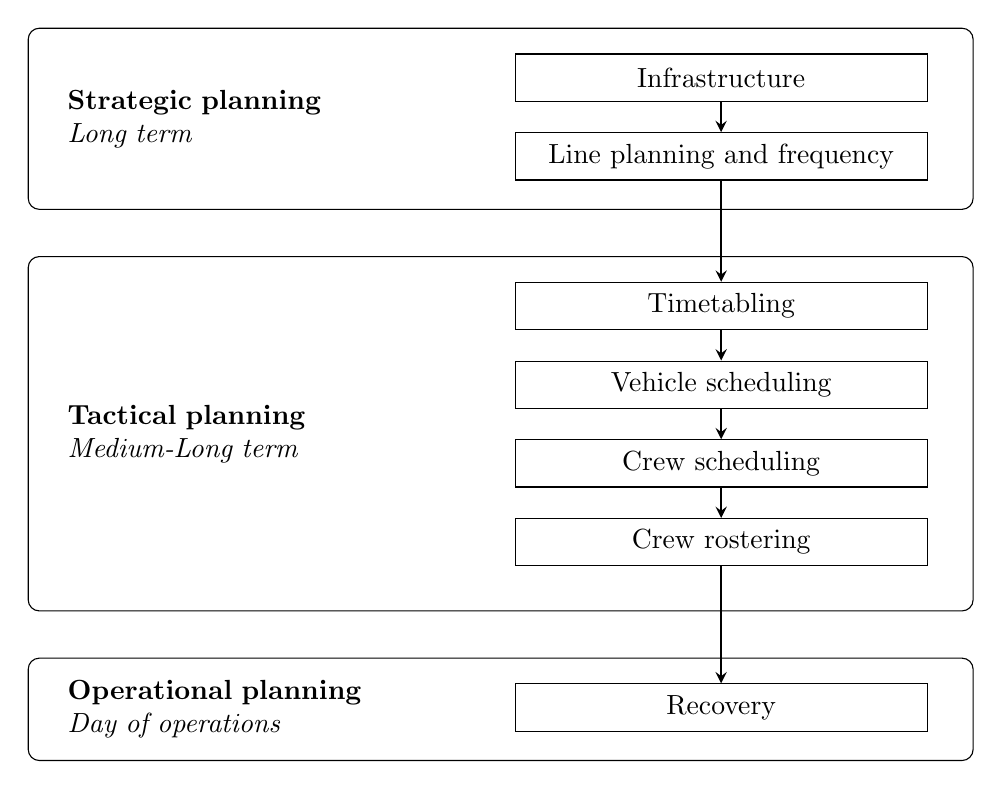
\begin{tikzpicture}[node distance=2cm]
  \node (strategic) [process, minimum height=2.3cm] {\textbf{Strategic planning}\\\textit{Long term}};
  \node at (strategic.base) (infra) [subprocess, xshift=2.8cm, yshift=0.4cm] {Infrastructure};
  \node at (strategic.base) (line) [subprocess, below of=infra, yshift=1cm] {Line planning and frequency};
  
  \node (tactical) [process, minimum height=4.5cm, below of=strategic, yshift=-2cm] {\textbf{Tactical planning}\\\textit{Medium-Long term}};
  \node at (tactical.base) (timetable) [subprocess, xshift=2.8cm, yshift=1.5cm] {Timetabling};
  \node at (tactical.base) (vehicle) [subprocess, below of=timetable, yshift=1cm] {Vehicle scheduling};
  \node at (tactical.base) (crew) [subprocess, below of=vehicle, yshift=1cm] {Crew scheduling};
  \node at (tactical.base) (rostering) [subprocess, below of=crew, yshift=1cm] {Crew rostering};

  \node (operational) [process, minimum height=1.3cm, below of=tactical, yshift=-1.5cm] {\textbf{Operational planning}\\\textit{Day of operations}};
  \node at (operational.base) (recovery) [subprocess, xshift=2.8cm, yshift=-0.1cm] {Recovery};


  \draw [arrow] (infra) -- (line);
  \draw [arrow] (line) -- (timetable);
  \draw [arrow] (timetable) -- (vehicle);
  \draw [arrow] (vehicle) -- (crew);
  \draw [arrow] (crew) -- (rostering);
  \draw [arrow] (rostering) -- (recovery);
\end{tikzpicture}
\caption{A general overview of the public transport planning process, based on \cite{IBARRAROJAS201538}, \cite{PERUMAL2022395}.}
\label{fig:planning-overview}
\end{figure}


\section{Related work}
In this section, we will discuss work related to our research into the E-VSCP.  An overview of the modeling of batteries in E-VS(C)P approaches has also been included in Table \ref{tab:evscp-lit}.  \\\\ 
\noindent \textbf{(E-)VSP} \\\\
The Single Depot Vehicle Scheduling Problem (SDVSP) has long been known to be polynomially solvable, however the inclusion of multiple depots has been shown to make the problem NP-hard under the assumption that busses must return to the same depot from which they originated \cite{Bunte2009}. Additionally, the introduction of any resource constraints such as limited ranges within the vehicle scheduling problem (VSP-RC) has also been shown to be NP-hard by Bodin et al. \cite{BODIN198363}. As the E-VSP inherently must deal with the limited range associated with electric vehicles, this problem is also NP-hard as shown by Oulamara and Sassi \cite{Sassi2014}. \\\\
\todo{meer info} van Kooten Niekerk et al. introduce a pair of models which aim to solve the E-VSP while taking into account time of use pricing, nonlinear charging times and battery degredation due to depth of decharge \cite{vanKootenNiekerk2017}. They do this by extending the graph underlying the traditional VSP using either continuous state of charge variables or discrete trip nodes modeling state of charge, and solve using Column Generation (CG). They test using data provided by Belgian company De Lijn, using a total of 543 trips. They show that the discretized model can be solved in a shorter timeframe with similar results to the continuous model. \\\\
Jiang et al. use a Large Neighbourhood Search (LNS) approach to solve the E-VSP \cite{Jiang2021}. They consider time of use energy costs and opportunisitic charging. They use test data in Shenzhen, China with a total of 778 trips. \todo{meer info maar de paper is saai}.


\noindent \textbf{(E-)VSCP} \todo{Deze kopjes erin houden? Of gwn weghalen.} \\

As far as we are aware, only four other works discuss the E-VSCP. Perumal et al. were the first to offer a solution to the E-VSCP in 2021 \cite{PERUMAL2021105268}. They introduced an Adaptive Large Neighbourhood Search (ALNS) which incorporates a Branch \& Price (B\&P) hueristic which has been previously used to solve the multi-depot VSP, E-VSP and VCSP \cite{Pepin2009, Haase1996, vanKootenNiekerk2017}. Additionally, they adapt an embedding of a B\&P hueristic into the ALNS as introduced by Pepin et al. \cite{Pepin2009}. They only consider full recharges with a fixed duration of 120 minutes, charging at the depot and fixed maximum ranges for vehicles. The authors tested using real life data from lines in Denmark and Sweden with a maximum instance size of 1109 trips, and report an improvement of $1.17-4.37\%$ across different instances when compared to a sequential approach. \\
Sistig and Sauer also offered a ALNS based approach in 2023, which aimed to include partial recharges, opportunisitic charging at terminal stops of trips and non-fixed ranges for the vehicles \cite{SISTIG2023120915}. \todo{dit is niet interessant. This ALNS extends a previous LNS by Shaw which was aimed at the more general vehicle routing problem \cite{Shaw1997ANL, Shaw1998ANL}.} Tests were done using an instance of a city route in Germany, with a total of 282 trips. Different scenarios based on possible crew break and relief locations were considered in order to compare diesel and electric total cost of ownership. \\
Wang et al. introduce a two layered model using particle swarms and a $\epsilon$-constraint based mechanism which allows for a mix of diesel and electric busses \cite{su14063627}. The model incorporates partial depot charging, as well as measures to ensure that crew is primarily assigned the same vehicle type. A circular bus route in China with 68 daily trips is used as a basis for testing, with a focus on electric versus diesel usage and driver satisfaction. \\
Shen and Li provide a minimum-cost flow framework for the E-VSP which is integrated with a set partitioning based approach for the E-CSP \cite{SHEN2023}. They only provide full recharge capabilities at the depot, however focus on the inclusion of a distinction between driving and standstill time of vehicles in order to more accurately model real life traffic. A city line in China with 270 daily trips is used for testing, resulting in cost savings of up to 8.7\% when compared to a sequential approach.

\begin{table}[h]
  \centering
  \begin{tabular}{cllllll}
      \toprule
      & Model & ToU & SoC & Partial charging & Charge location & Degredation \\
      \cmidrule(lr){2-7}
      \cite{vanKootenNiekerk2017} & E-VSP & Yes & C/D & Yes & D/O & Yes \\
      \cite{Jiang2021} & E-VSP & Yes & C & Yes & O & No \\ 
      \cite{PERUMAL2021105268} & E-VSCP & No & C & No & D & No  \\
      \cite{SISTIG2023120915} & E-VSCP & No & C & Yes & D/O & No \\
      \cite{su14063627} & E-VSCP & Yes & C & Yes & D & No \\
      \cite{SHEN2023} & E-VSCP & No & C & No & D/O & No \\
      \bottomrule
  \end{tabular}
  \caption{A brief overview of battery modeling in E-VSP and E-VSCP literature. ToU = time of use electricity prices, State of charge (SoC) is either modeled as a (D)iscrete or (C)ontinuous variable, Partial charging yes/no, charge location (D)epot, (O)pportunity, (I)n motion, Degredation in cost function}
  \label{tab:evscp-lit}
\end{table}

\section{Problem definition}
Let $T$ be a set of trips that needs to be run. 
\printbibliography
\end{document}